\documentclass[10pt,t]{beamer} 
\usepackage[utf8]{inputenc}
\usepackage[T1]{fontenc}
\fontfamily{ppl}\selectfont

\usepackage{fontspec} 
\defaultfontfeatures{Mapping=tex-text} 
\setsansfont[Ligatures={Common}]{Futura}
\setmonofont[Scale=0.8]{Monaco} 



%\setbeamersize{text margin left=10pt,text margin right=10pt}
\usetheme{lehigh}

\usefonttheme{professionalfonts}
\usefonttheme{serif}

\pgfdeclarelayer{background}
\pgfdeclarelayer{foreground}
\pgfsetlayers{background,main,foreground}

% add packages to use
%\usepackage[latin1]{inputenc}
%\usepackage[english]{babel}
%\usepackage[normalem]{ulem}
\usepackage{times}
\usepackage[T1]{fontenc}
\usepackage{pgf,pgfarrows,pgfnodes,pgfautomata,pgfheaps,pgfshade}
\usepackage{amsmath,amssymb,amsfonts,subfigure,pifont}
\usepackage{graphicx}
\usepackage{multirow,multicol}
\usepackage{tabularx}
\usepackage{booktabs}
\usepackage{colortbl}
\usepackage{fancyvrb,listings}
\usepackage{algorithm,algpseudocode}
%\usepackage{keystroke}
\usepackage{etex}
\usepackage{hyperref}
\usepackage{tikz}
\usetikzlibrary{trees,matrix,shapes,arrows}
\usetikzlibrary{calc}



% The following color are for listing environment 
\definecolor{dkgreen}{rgb}{0,0.6,0}
\definecolor{DarkGreen}{rgb}{0.0,0.3,0.0}
\definecolor{gray}{rgb}{0.5,0.5,0.5}
\definecolor{mauve}{rgb}{0.58,0,0.82}
\definecolor{Blue}{rgb}{0.0,0.0,0.8} 
\definecolor{dodgerblue}{rgb}{0.1,0.1,1.0}
\definecolor{indigo}{rgb}{0.41,0.1,0.0}
\definecolor{seagreen}{rgb}{0.1,1.0,0.1}


\lstset{%
language=bash,                % the language of the code
basicstyle=\tiny\ttfamily,           % the size of the fonts that are used for the code
showspaces=false,               % show spaces adding particular underscores
showstringspaces=false,         % underline spaces within strings
showtabs=false,                 % show tabs within strings adding particular underscores
%frame=single,                   % adds a frame around the code
%rulecolor=\color{black},        % if not set, the frame-color may be changed on line-breaks within not-black text (e.g. comments (green here))
tabsize=2,                      % sets default tabsize to 2 spaces
%captionpos=b,                   % sets the caption-position to bottom
breaklines=true,                % sets automatic line breaking
breakatwhitespace=false,        % sets if automatic breaks should only happen at whitespace
%title=\lstname,                   % show the filename of files included with \lstinputlisting;
% also try caption instead of title
keywordstyle=\color{blue},          % keyword style
commentstyle=\color{dkgreen},       % comment style
stringstyle=\color{mauve},         % string literal style
escapeinside={!}{!},            % if you want to add LaTeX within your code
morekeywords={*,\dots,elif},              % if you want to add more keywords to the set
deletekeywords={\dots},              % if you want to delete keywords from the given language
%morecomment=[l]{//}
}
\lstset{%
language=csh,                % the language of the code
basicstyle=\tiny\ttfamily,           % the size of the fonts that are used for the code
showspaces=false,               % show spaces adding particular underscores
showstringspaces=false,         % underline spaces within strings
showtabs=false,                 % show tabs within strings adding particular underscores
%frame=single,                   % adds a frame around the code
%rulecolor=\color{black},        % if not set, the frame-color may be changed on line-breaks within not-black text (e.g. comments (green here))
tabsize=2,                      % sets default tabsize to 2 spaces
captionpos=b,                   % sets the caption-position to bottom
breaklines=true,                % sets automatic line breaking
breakatwhitespace=false,        % sets if automatic breaks should only happen at whitespace
%title=\lstname,                   % show the filename of files included with \lstinputlisting;
% also try caption instead of title
keywordstyle=\color{blue},          % keyword style
commentstyle=\color{dkgreen},       % comment style
stringstyle=\color{mauve},         % string literal style
escapeinside={\%*}{*)},            % if you want to add LaTeX within your code
morekeywords={*,\dots,elif},              % if you want to add more keywords to the set
deletekeywords={\dots},              % if you want to delete keywords from the given language
%morecomment=[l]{//}
}

\lstdefinestyle{LINUX}
{
    backgroundcolor=\color{white},
    basicstyle=\tiny\ttfamily,
    keywordstyle=\color{blue},
    morekeywords={apacheco,Tutorials,BASH,scripts,day1,examples},
    literate={>}{{\textcolor{blue}{>}}}1
         {/}{{\textcolor{blue}{/}}}1
         {./}{{\textcolor{black}{./ }}}1
         {~}{{\textcolor{blue}{\textasciitilde}}}1,
}

\lstdefinestyle{customc}{
  belowcaptionskip=1\baselineskip,
  breaklines=true,
  xleftmargin=\parindent,
  language=C,
  showstringspaces=false,
  basicstyle=\tiny\ttfamily,
  keywordstyle=\bfseries\color{green!40!black},
  commentstyle=\upshape\color{red!90!white},
  identifierstyle=\color{blue},
  stringstyle=\color{orange},
}
\lstdefinelanguage{OmpFortran}[]{Fortran}{
   rulesepcolor=\color{black},
   %
   extendedchars=true,
   %
   morecomment=[l] [\bfseries\color{red!90!white}]{!\$omp},
   morecomment=[l] [\bfseries\color{red!90!white}]{c\$omp},
   morecomment=[l] [\bfseries\color{red!90!white}]{*\$omp},
   morecomment=[l] [\bfseries\color{red!90!white}]{!\$acc},
   morecomment=[l] [\bfseries\color{red!90!white}]{c\$acc},
   morecomment=[l] [\bfseries\color{red!90!white}]{*\$acc},
}[comments]

\lstdefinelanguage{OmpC}[]{OmpFortran}{
   rulesepcolor=\color{black},
   %
   extendedchars=true,
   %
   morecomment=[l] [\bfseries\color{red!90!white}]{\#pragma\ omp},
   morecomment=[l] [\bfseries\color{red!90!white}]{\#pragma\ acc},
}[comments]

\lstset{escapechar=@,style=customc}
\lstset{literate=%
   *{0}{{{\color{blue}0}}}1
    {1}{{{\color{blue}1}}}1
    {2}{{{\color{blue}2}}}1
    {3}{{{\color{blue}3}}}1
    {4}{{{\color{blue}4}}}1
    {5}{{{\color{blue}5}}}1
    {6}{{{\color{blue}6}}}1
    {7}{{{\color{blue}7}}}1
    {8}{{{\color{blue}8}}}1
    {9}{{{\color{blue}9}}}1
}

\algrenewcommand\algorithmicfunction{\textbf{program}}
\algblockdefx[Program]{Program}{EndProgram}[1]{\textbf{program} \textsc{#1}}[1]{\textbf{end program} \textsc{#1}}
\algloopdefx[doloop]{Do}[1]{\textbf{do} #1}
\algcblockdefx[doloop]{If}{Do}{EndDo}
[1]{\textbf{do} #1}{\textbf{end do}}


\DeclareSymbolFont{extraup}{U}{zavm}{m}{n}
%\DeclareMathSymbol{\vardiamond}{\mathalpha}{extraup}{87}
\newcommand{\cmark}{\ding{51}}
\newcommand{\xmark}{\ding{55}}
\newcommand{\smark}{\ding{77}}
\newcommand*\vardiamond{\textcolor{lubrown}{%
  \ensuremath{\blacklozenge}}}
\newcommand*\mybigstar{\textcolor{lubrown!90!yellow}{%
  \ensuremath{\bigstar}}}
\newcommand*\up{\textcolor{green!80!black}{%
  \ensuremath{\blacktriangle}}}
\newcommand*\down{\textcolor{red}{%
  \ensuremath{\blacktriangledown}}}
\newcommand*\const{\textcolor{darkgray}%
  {\textbf{--}}}
\newcommand*\enter{\tikz[baseline=-0.5ex] \draw[<-] (0,0) -| (0.5,0.1);}
\newcommand{\bftt}[1]{\textbf{\texttt{#1}}}
\newcommand{\bflub}[1]{\textbf{\color{lubrown}#1}}
\newcommand{\lstfortran}[1]{\lstinline[language={[90]Fortran},basicstyle=\small\ttfamily]|#1|}
\newcommand{\lstC}[1]{\lstinline[language=C,basicstyle=\small\ttfamily]|#1|}
\newcommand{\Verblubrown}[1]{\Verb[formatcom=\color{lubrown},fontseries=b,commandchars=\\\{\}]|#1|}
\newcommand{\Verblue}[1]{\Verb[formatcom=\color{lublue},fontseries=b,commandchars=\\\{\}]!#1!}
\newcommand{\Verbblue}[2][b]{\Verb[formatcom=\color{lublue},fontshape=#1,commandchars=\\\{\}]|#2|}
\newcommand{\Verblubrownp}[1]{\Verb[formatcom=\color{lubrown},fontseries=b,commandchars=\\\{\}]!#1!}
\newcommand{\Verbred}[1]{\Verb[formatcom=\color{red},commandchars=\\\{\}]|#1|}
\newcommand{\Verbindigo}[1]{\Verb[formatcom=\color{indigo},fontsize=\fontsize{7.5}{8}\selectfont,commandchars=\\\{\}]!#1!}

\newcolumntype{a}{>{\columncolor{lulime}}c}
\newcolumntype{b}{>{\columncolor{lulime!50}}c}
\newcolumntype{d}{>{\columncolor{lulime!40}}c}
\newcolumntype{e}{>{\columncolor{lulime}}l}
\newcolumntype{f}{>{\columncolor{lulime!50}}l}

                           
% LOGOS
\pgfdeclareimage[height=0.55cm]{lucolor-logo}{LehighU_official-logo_Color.png}
\rplogo{\pgfuseimage{lucolor-logo}}
\pgfdeclareimage[height=0.55cm]{luwhite-logo}{LehighU_official-logo_White.png}
\tplogo{\pgfuseimage{luwhite-logo}}
% footer logo
%\pgfdeclareimage[width=0.3\paperwidth]{university-logo}{lulogo}
%\tllogo{\pgfuseimage{university-logo}}

%titlepage logo
%\titlegraphic{
\includegraphics[scale=0.5]{lu}}

\beamertemplateballitem



\title[MPI]{Introduction to MPI}
\subtitle{2021~HPC~Workshop:~Parallel~Programming}
\author{\large{Alexander~B.~Pacheco}}
\institute[Lehigh University Research Computing]{\href{http://researchcomputing.lehigh.edu}{Research~Computing}}
\date{July~13~-~15,~2021}
    
\AtBeginSection[]
{
  \begingroup
%  \setbeamertemplate{background canvas}[vertical shading][bottom=lubrown,top=lubrown]
%  \setbeamertemplate{footline}[myfootline] 
%  \setbeamertemplate{section page}[mysection]
  \frame[c]{
%    \sectionpage
    \tableofcontents[currentsection,currentsubsection]
  }
  \endgroup
}

\begin{document}

\begin{frame}
  \titlepage
\end{frame}

\scriptsize
\section{Introduction}
\begin{frame}
  \frametitle{Distributed Memory Model}
%  \begin{columns}
%    \column{6cm}
    \begin{itemize}
      \item Each process has its own address space
      \begin{itemize}
        \item Data is local to each process
      \end{itemize}
      \item Data sharing is achieved via explicit message passing
      \item Example
      \begin{itemize}
        \item MPI
      \end{itemize}
    \end{itemize}
%    \column{6cm}
%    \begin{center}
%      \includegraphics[width=8cm]{./distributed}
%    \end{center}
%  \end{columns}
%\end{frame}

%\begin{frame}
    \begin{center}
      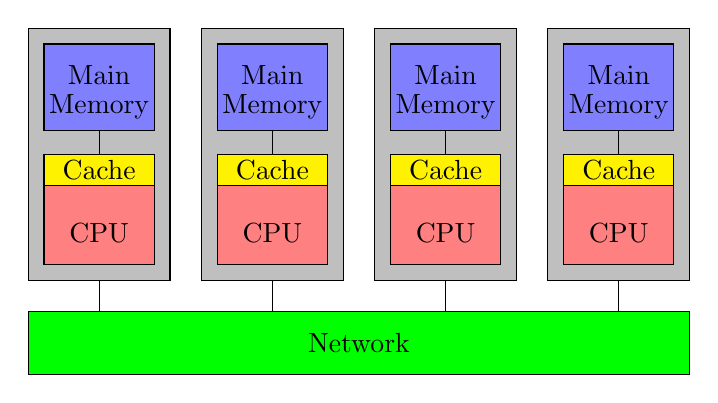
\begin{tikzpicture}[scale=0.4]
        \filldraw[fill=green] (0,-1) rectangle (21,-3);
        \draw (10.5,-2.0) node {Network};
        % First Node
        \filldraw[fill=gray!50!white] (0,0) rectangle (4.5,8);
        \filldraw[fill=blue!50!white] (0.5,4.75) rectangle (4.0,7.5);
        \filldraw[fill=yellow] (0.5,3.0) rectangle (4.0,4,0);
        \filldraw[fill=red!50!white] (0.5,0.5) rectangle (4.0,3.0);
        \draw (2.25,4.0) -- (2.25,4.75);
        \draw (2.25,0) -- (2.25,-1);
        \draw (2.25,6.5) node {Main};
        \draw (2.25,5.5) node {Memory};
        \draw (2.25,1.5) node {CPU};
        \draw (2.25,3.5) node {Cache};
        
        % Second Node
        \filldraw[fill=gray!50!white] (5.5,0) rectangle (10.0,8);
        \filldraw[fill=blue!50!white] (6.0,4.75) rectangle (9.5,7.5);
        \filldraw[fill=yellow] (6.0,3.0) rectangle (9.5,4,0);
        \filldraw[fill=red!50!white] (6.0,0.5) rectangle (9.5,3.0);
        \draw (7.75,4.0) -- (7.75,4.75);
        \draw (7.75,0) -- (7.75,-1);
        \draw (7.75,6.5) node {Main};
        \draw (7.75,5.5) node {Memory};
        \draw (7.75,1.5) node {CPU};
        \draw (7.75,3.5) node {Cache};
        
        % Third Node
        \filldraw[fill=gray!50!white] (11.0,0) rectangle (15.5,8);
        \filldraw[fill=blue!50!white] (11.5,4.75) rectangle (15.0,7.5);
        \filldraw[fill=yellow] (11.5,3.0) rectangle (15.0,4,0);
        \filldraw[fill=red!50!white] (11.5,0.5) rectangle (15.0,3.0);
        \draw (13.25,4.0) -- (13.25,4.75);
        \draw (13.25,0) -- (13.25,-1);
        \draw (13.25,6.5) node {Main};
        \draw (13.25,5.5) node {Memory};
        \draw (13.25,1.5) node {CPU};
        \draw (13.25,3.5) node {Cache};
        
        % Fourth Node
        \filldraw[fill=gray!50!white] (16.5,0) rectangle (21.0,8);
        \filldraw[fill=blue!50!white] (17.0,4.75) rectangle (20.5,7.5);
        \filldraw[fill=yellow] (17.0,3.0) rectangle (20.5,4,0);
        \filldraw[fill=red!50!white] (17.0,0.5) rectangle (20.5,3.0);
        \draw (18.75,4.0) -- (18.75,4.75);
        \draw (18.75,0) -- (18.75,-1);
        \draw (18.75,6.5) node {Main};
        \draw (18.75,5.5) node {Memory};
        \draw (18.75,1.5) node {CPU};
        \draw (18.75,3.5) node {Cache};
      \end{tikzpicture}
    \end{center}
\end{frame}

\begin{frame}
  \frametitle{Shared Memory Model}
%  \begin{columns}
%    \column{6cm}
    \begin{itemize}
      \item All threads can access the global memory space.
      \item Data sharing achieved via writing to/reading from the same memory location
      \item Example
      \begin{itemize}
        \item OpenMP
        \item Pthreads
      \end{itemize}
    \end{itemize}
%    \column{6cm}
    \begin{center}
      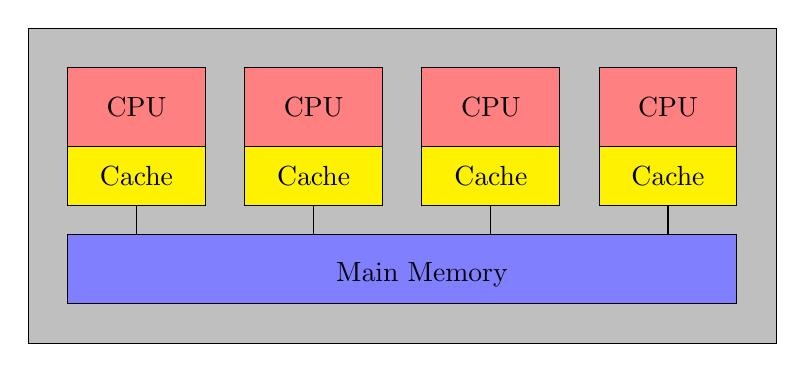
\begin{tikzpicture}[scale=0.5]
        \filldraw[fill=gray!50!white] (0,0) rectangle (19,8);
        \filldraw[fill=blue!50!white] (1,1) rectangle (18,2.75);
        \draw (10,1.75) node {Main Memory};
        % First Core
        \filldraw[fill=yellow] (1,3.5) rectangle (4.5,5.0);
        \draw (2.75,4.25) node {Cache};
        \filldraw[fill=red!50!white] (1,5.0) rectangle (4.5,7.0);
        \draw (2.75,6.0) node {CPU};
        \draw (2.75,3.5) -- (2.75,2.75);
        % Second Core
        \filldraw[fill=yellow] (5.5,3.5) rectangle (9.0,5.0);
        \draw (7.25,4.25) node {Cache};
        \filldraw[fill=red!50!white] (5.5,5.0) rectangle (9.0,7.0);
        \draw (7.25,6.0) node {CPU};
        \draw (7.25,3.5) -- (7.25,2.75);
        % Third Core
        \filldraw[fill=yellow] (10.0,3.5) rectangle (13.5,5.0);
        \draw (11.75,4.25) node {Cache};
        \filldraw[fill=red!50!white] (10.0,5.0) rectangle (13.5,7.0);
        \draw (11.75,6.0) node {CPU};
        \draw (11.75,3.5) -- (11.75,2.75);
        % Fourth Core
        \filldraw[fill=yellow] (14.5,3.5) rectangle (18.0,5.0);
        \draw (16.25,4.25) node {Cache};
        \filldraw[fill=red!50!white] (14.5,5.0) rectangle (18.0,7.0);
        \draw (16.25,6.0) node {CPU};
        \draw (16.25,3.5) -- (16.25,2.75);
      \end{tikzpicture}
%      \includegraphics[width=8cm]{./shared}
    \end{center}
%  \end{columns}
\end{frame}


\begin{frame}
  \frametitle{Clusters of SMP nodes}
  \begin{itemize}
    \item The shared memory model is most commonly represented by Symmetric Multi-Processing (SMP) systems
    \begin{itemize}
      \item Identical processors
      \item Equal access time to memory
    \end{itemize}
    \item Large shared memory systems are rare, clusters of SMP nodes are popular.
  \end{itemize}
%  \begin{columns}
%    \column{13cm}
%    \begin{center}
%      \includegraphics[width=12cm]{./smp-cluster}
%    \end{center}
%  \end{columns}
%\end{frame}

%\begin{frame}
  \begin{center}
    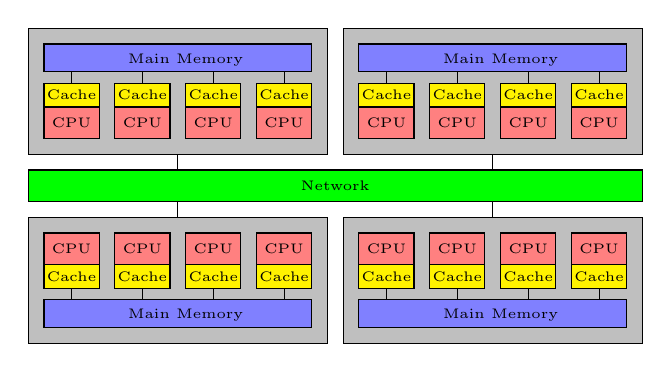
\begin{tikzpicture}[scale=0.2]
      \tikzstyle{every node}=[font=\tiny]
      \filldraw[fill=green] (0,9) rectangle (39,11);
      \draw (19.5,10) node {Network};
      % First Node
      \filldraw[fill=gray!50!white] (0,0) rectangle (19,8);
      \filldraw[fill=blue!50!white] (1,1) rectangle (18,2.75);
      \draw (10,1.75) node {Main Memory};
      % First Core
      \filldraw[fill=yellow] (1,3.5) rectangle (4.5,5.0);
      \draw (2.75,4.25) node {Cache};
      \filldraw[fill=red!50!white] (1,5.0) rectangle (4.5,7.0);
      \draw (2.75,6.0) node {CPU};
      \draw (2.75,3.5) -- (2.75,2.75);
      % Second Core
      \filldraw[fill=yellow] (5.5,3.5) rectangle (9.0,5.0);
      \draw (7.25,4.25) node {Cache};
      \filldraw[fill=red!50!white] (5.5,5.0) rectangle (9.0,7.0);
      \draw (7.25,6.0) node {CPU};
      \draw (7.25,3.5) -- (7.25,2.75);
      % Third Core
      \filldraw[fill=yellow] (10.0,3.5) rectangle (13.5,5.0);
      \draw (11.75,4.25) node {Cache};
      \filldraw[fill=red!50!white] (10.0,5.0) rectangle (13.5,7.0);
      \draw (11.75,6.0) node {CPU};
      \draw (11.75,3.5) -- (11.75,2.75);
      % Fourth Core
      \filldraw[fill=yellow] (14.5,3.5) rectangle (18.0,5.0);
      \draw (16.25,4.25) node {Cache};
      \filldraw[fill=red!50!white] (14.5,5.0) rectangle (18.0,7.0);
      \draw (16.25,6.0) node {CPU};
      \draw (16.25,3.5) -- (16.25,2.75);
      % Connect First Node to Network
      \draw (9.5,8) -- (9.5,9);

      % Second Node
      \filldraw[fill=gray!50!white] (20,0) rectangle (39,8);
      \filldraw[fill=blue!50!white] (21,1) rectangle (38,2.75);
      \draw (30,1.75) node {Main Memory};
      % First Core
      \filldraw[fill=yellow] (21,3.5) rectangle (24.5,5.0);
      \draw (22.75,4.25) node {Cache};
      \filldraw[fill=red!50!white] (21,5.0) rectangle (24.5,7.0);
      \draw (22.75,6.0) node {CPU};
      \draw (22.75,3.5) -- (22.75,2.75);
      % Second Core
      \filldraw[fill=yellow] (25.5,3.5) rectangle (29.0,5.0);
      \draw (27.25,4.25) node {Cache};
      \filldraw[fill=red!50!white] (25.5,5.0) rectangle (29.0,7.0);
      \draw (27.25,6.0) node {CPU};
      \draw (27.25,3.5) -- (27.25,2.75);
      % Third Core
      \filldraw[fill=yellow] (30.0,3.5) rectangle (33.5,5.0);
      \draw (31.75,4.25) node {Cache};
      \filldraw[fill=red!50!white] (30.0,5.0) rectangle (33.5,7.0);
      \draw (31.75,6.0) node {CPU};
      \draw (31.75,3.5) -- (31.75,2.75);
      % Fourth Core
      \filldraw[fill=yellow] (34.5,3.5) rectangle (38.0,5.0);
      \draw (36.25,4.25) node {Cache};
      \filldraw[fill=red!50!white] (34.5,5.0) rectangle (38.0,7.0);
      \draw (36.25,6.0) node {CPU};
      \draw (36.25,3.5) -- (36.25,2.75);
      % Connect Second Node to Network
      \draw (29.5,8) -- (29.5,9);

      % Third Node
      \filldraw[fill=gray!50!white] (0,12) rectangle (19,20);
      \filldraw[fill=blue!50!white] (1,17.25) rectangle (18,19);
      \draw (10,18.0) node {Main Memory};
      % First Core
      \filldraw[fill=yellow] (1,16.5) rectangle (4.5,15.0);
      \draw (2.75,15.75) node {Cache};
      \filldraw[fill=red!50!white] (1,15.0) rectangle (4.5,13.0);
      \draw (2.75,14.0) node {CPU};
      \draw (2.75,16.5) -- (2.75,17.25);
      % Second Core 
      \filldraw[fill=yellow] (5.5,16.5) rectangle (9.0,15.0);
      \draw (7.25,15.75) node {Cache};
      \filldraw[fill=red!50!white] (5.5,15.0) rectangle (9.0,13.0);
      \draw (7.25,14.0) node {CPU};
      \draw (7.25,16.5) -- (7.25,17.25);
      % Third Core 
      \filldraw[fill=yellow] (10.0,16.5) rectangle (13.5,15.0);
      \draw (11.75,15.75) node {Cache};
      \filldraw[fill=red!50!white] (10.0,15.0) rectangle (13.5,13.0);
      \draw (11.75,14.0) node {CPU};
      \draw (11.75,16.5) -- (11.75,17.25);
      % Fourth Core 
      \filldraw[fill=yellow] (14.5,16.5) rectangle (18.0,15.0);
      \draw (16.25,15.75) node {Cache};
      \filldraw[fill=red!50!white] (14.5,15.0) rectangle (18.0,13.0);
      \draw (16.25,14.0) node {CPU};
      \draw (16.25,16.5) -- (16.25,17.25);
      % Connect Third Node to Network
      \draw (9.5,11) -- (9.5,12);

      % Fourth Node
      \filldraw[fill=gray!50!white] (20,12) rectangle (39,20);
      \filldraw[fill=blue!50!white] (21,17.25) rectangle (38,19);
      \draw (30,18.0) node {Main Memory};
      % First Core
      \filldraw[fill=yellow] (21,16.5) rectangle (24.5,15.0);
      \draw (22.75,15.75) node {Cache};
      \filldraw[fill=red!50!white] (21,15.0) rectangle (24.5,13.0);
      \draw (22.75,14.0) node {CPU};
      \draw (22.75,16.5) -- (22.75,17.25);
      % Second Core 
      \filldraw[fill=yellow] (25.5,16.5) rectangle (29.0,15.0);
      \draw (27.25,15.75) node {Cache};
      \filldraw[fill=red!50!white] (25.5,15.0) rectangle (29.0,13.0);
      \draw (27.25,14.0) node {CPU};
      \draw (27.25,16.5) -- (27.25,17.25);
      % Third Core 
      \filldraw[fill=yellow] (30.0,16.5) rectangle (33.5,15.0);
      \draw (31.75,15.75) node {Cache};
      \filldraw[fill=red!50!white] (30.0,15.0) rectangle (33.5,13.0);
      \draw (31.75,14.0) node {CPU};
      \draw (31.75,16.5) -- (31.75,17.25);
      % Fourth Core 
      \filldraw[fill=yellow] (34.5,16.5) rectangle (38.0,15.0);
      \draw (36.25,15.75) node {Cache};
      \filldraw[fill=red!50!white] (34.5,15.0) rectangle (38.0,13.0);
      \draw (36.25,14.0) node {CPU};
      \draw (36.25,16.5) -- (36.25,17.25);
      % Connect Fourth Node to Network
      \draw (29.5,11) -- (29.5,12);
      
    \end{tikzpicture}
  \end{center}
\end{frame}

\begin{frame}
  \frametitle{Shared vs Distributed}
%  \begin{columns}
%    \column{5cm}
    \begin{exampleblock}{Shared Memory}
      \begin{itemize}
        \item Pros
        \begin{itemize}
          \item Global address space is user friendly
          \item Data sharing is fast
        \end{itemize}
        \item Cons
        \begin{itemize}
          \item Lack of scalability
          \item Data conflict issues
        \end{itemize}
      \end{itemize}
    \end{exampleblock}
%    \column{5cm}
    \begin{exampleblock}{Distributed Memory}
      \begin{itemize}
        \item Pros
        \begin{itemize}
          \item Memory scalable with number of processors
          \item Easier and cheaper to build
        \end{itemize}
        \item Cons
        \begin{itemize}
          \item Difficult load balancing
          \item Data sharing is slow
        \end{itemize}
      \end{itemize}
    \end{exampleblock}
%  \end{columns}
\end{frame}

\begin{frame}
  \frametitle{Why MPI?}
  \begin{itemize}
    \item There are already network communication libraries
    \item Optimized for performance
    \item Take advantage of faster network transport
      \begin{itemize}
        \item Shared memory (within a node)
        \item Faster cluster interconnects (e.g. InfiniBand)
        \item TCP/IP if all else fails
      \end{itemize}
    \item Enforces certain guarantees
      \begin{itemize}
      \item Reliable messages
      \item In-order message arrival
      \end{itemize}
    \item Designed for multi-node technical computing
  \end{itemize}
\end{frame}

\begin{frame}
  \frametitle{What is MPI?}
  \begin{itemize}
    \item MPI defines a standard API for message passing
      \begin{itemize}
        \item The standard includes
          \begin{itemize}
          \item What functions are available
          \item The syntax of those functions
          \item What the expected outcome is when calling those functions
          \end{itemize}
        \item The standard does NOT include
          \begin{itemize}
            \item Implementation details (e.g. how the data transfer occurs)
            \item Runtime details (e.g. how many processes the code run with  etc.)
          \end{itemize}
      \end{itemize}
    \item MPI provides C/C++ and Fortran bindings
  \end{itemize}
\end{frame}

\begin{frame}
  \frametitle{MPI Implementations}
  \begin{itemize}
    \item There are two different types of MPI implementations commonly used. 
    \begin{enumerate}
       \item {\bf MPICH}: Developed by Argonne National Laboratory.
       \begin{itemize}
           \item used as a starting point for various commercial and open source MPI libraries
           \item {\bf MVAPICH2}: Developed by D. K. Panda with support for  InfiniBand, iWARP, RoCE, and Intel Omni-Path. (default MPI on Sol),
           \item {\bf Intel MPI}: Intel's version of MPI. Part of Intel OneAPI HPC Toolkit
           \item {\bf IBM MPI}:  for IBM BlueGene, and 
           \item {\bf CRAY MPI}: for Cray systems.
       \end{itemize}
       \item {\bf OpenMPI}: A Free, Open Source implementation from merger of three well know MPI implementations. Can be used for commodity network as well as high speed network.
       \begin{itemize}
           \item {\bf FT-MPI} from the University of Tennessee,
           \item {\bf LA-MPI}: from Los Alamos National Laboratory,
           \item {\bf LAM/MPI}: from Indiana University
       \end{itemize}
    \end{enumerate}
  \end{itemize}
\end{frame}

\begin{frame}[fragile]
  \frametitle{MPI Compilers}
  \begin{itemize}
    \item There is no MPI compiler available to compile programs nor is there is a compiler flag.
    \item Instead, you need to build the MPI scripts for a particular compiler.
    \item You can use MVAPICH2 and MPICH on Sol
    \item You should use MPICH only on Hawk. 
    \item Each of these builds provide mpicc, mpicxx and mpif90 for compiling C, C++ and Fortran codes respectively that are wrapper for the underlying compilers
  \end{itemize}
  \begin{lstlisting}[basicstyle=\tiny\ttfamily]
[alp514.sol](793): module load mvapich2
[alp514.sol](794): mpicc -show
/share/Apps/intel/2020/compilers_and_libraries_2020.3.275/linux/bin/intel64/icc -lmpi -I/share/Apps/lusoft/opt/spack/linux-centos8-haswell/intel-20.0.3/mvapich2/2.3.4-wguydha/include -L/share/Apps/lusoft/opt/spack/linux-centos8-haswell/intel-20.0.3/mvapich2/2.3.4-wguydha/lib -Wl,-rpath -Wl,/share/Apps/lusoft/opt/spack/linux-centos8-haswell/intel-20.0.3/mvapich2/2.3.4-wguydha/lib
[alp514.sol](795): module load mpich

Lmod is automatically replacing "mvapich2/2.3.4" with "mpich/3.3.2".

[alp514.sol](796): mpif90 -show
/share/Apps/intel/2020/compilers_and_libraries_2020.3.275/linux/bin/intel64/ifort -L/share/Apps/lusoft/opt/spack/linux-centos8-haswell/intel-20.0.3/hwloc/2.2.0-rjrzfy7/lib -I/share/Apps/lusoft/opt/spack/linux-centos8-haswell/intel-20.0.3/mpich/3.3.2-n7f36fo/include -I/share/Apps/lusoft/opt/spack/linux-centos8-haswell/intel-20.0.3/mpich/3.3.2-n7f36fo/include -L/share/Apps/lusoft/opt/spack/linux-centos8-haswell/intel-20.0.3/mpich/3.3.2-n7f36fo/lib -lmpifort -Wl,-rpath -Wl,/share/Apps/lusoft/opt/spack/linux-centos8-haswell/intel-20.0.3/mpich/3.3.2-n7f36fo/lib -lmpi
  \end{lstlisting}
\end{frame}

\begin{frame}[fragile,allowframebreaks]
  \frametitle{Running MPI Applications}
  \begin{itemize}
  \item To run MPI applications, you need to launch the application using mpirun (OpenMPI), mpirun\_rsh (MPICH and MVAPICH2) or mpiexec (OpenMPI, MPICH and MVAPICH2).
  \item mpirun, mpirun\_rsh and mpiexec are schedulers for the MPI library.
  \item On clusters with SLURM scheduler, srun can be used to launched MPI applications
  \item The MPI scheduler needs to be given additional information to correctly run MPI applications
  \end{itemize}
  \begin{center}
    \begin{tabular}{|faaa|}
      \hline
      \rowcolor{lublue}& mpiexec & mpirun\_rsh & mpirun \\
      \hline
      \# Processors & -n numprocs & -n numprocs & -np numprocs \\
      Processors List & -hosts core1,core2,... & core1 core2 ... & -hosts core1,core2,... \\
      Processor filelist & -f file & -hostfile file & -f/-hostfile file \\
      \hline
    \end{tabular}
  \end{center}
  \begin{itemize}
    \item Run an application myapp on 72 processors on a total of 3 nodes - node1, node2 and node3 
      \begin{itemize}
        \item mpirun: \lstinline|mpirun -np 72 -f filename myapp|
        \item mpirun\_rsh: \lstinline|mpirun_rsh -np 72 -hostfile filename myapp|
        \item mpiexec: \lstinline|mpiexec -n 72 -hosts node1,node2,node3 -ppn 24 myapp|
      \end{itemize}
  \end{itemize}
\end{frame}

\begin{frame}
  \frametitle{MPI Program Outline}
  \begin{enumerate}
    \item Initiate communication between processes
      \begin{itemize}
        \item {\bf \textcolor{lubrown}{MPI\_INIT}}: initialize MPI environment
        \item {\bf MPI\_COMM\_SIZE}: return total number of MPI processes
        \item {\bf MPI\_COMM\_RANK}: return rank of calling process
      \end{itemize}
      \item Communicate data between processes
        \begin{itemize}
          \item {\bf MPI\_SEND}: send a message
          \item {\bf MPI\_RECV}: receive a message 
        \end{itemize}
      \item Terminate the MPI environment using \textbf{\textcolor{lubrown}{MPI\_FINALIZE}}
  \end{enumerate}
\end{frame}

\begin{frame}{First MPI Program}
  \begin{columns}
    \column{0.45\textwidth}
    \begin{exampleblock}{C}
      \lstinputlisting[language=OmpC]{src/mpi/hello.c}
    \end{exampleblock}
    \column{0.45\textwidth}
    \begin{exampleblock}{Fortran}
      \lstinputlisting[language={OmpFortran}]{src/mpi/hello.f90}
    \end{exampleblock}
  \end{columns}
\end{frame}

\begin{frame}[fragile]
  \frametitle{Compile \& Run}
  \begin{exampleblock}{}
    \begin{lstlisting}
[alp514.sol](1003): module load mvapich2/2.2/intel-17.0.3
[alp514.sol](1004): mpicc -o helloc hello.c
[alp514.sol](1005): mpif90 -o hellof hello.f90
[alp514.sol](1006): srun -p eng -n 4 ./helloc
Number of tasks= 4 My rank= 3 Running on sol-b110
Number of tasks= 4 My rank= 2 Running on sol-b110
Number of tasks= 4 My rank= 1 Running on sol-b110
Number of tasks= 4 My rank= 0 Running on sol-b110
[alp514.sol](1007): srun -p eng -n 4 ./hellof
Number of tasks= 4 My rank= 3 Running on sol-b110
Number of tasks= 4 My rank= 2 Running on sol-b110
Number of tasks= 4 My rank= 0 Running on sol-b110
Number of tasks= 4 My rank= 1 Running on sol-b110
    \end{lstlisting}
  \end{exampleblock}
\end{frame}

\begin{frame}[fragile]
  \frametitle{MPI Program Structure}
  \begin{itemize}
    \item Header File: Required for all programs that make MPI library calls.
      \begin{center}
        \begin{tabular}{|a|a|}
          \hline
          \rowcolor{lublue}C & Fortran \\
          \hline
          \lstC{#include "mpi.h"} & \lstfortran{include 'mpif.h'} \\
          \hline
        \end{tabular}
      \end{center}
    \item Format of MPI Calls:
      \begin{itemize}
        \item C names are case sensitive; Fortran names are not.
        \item Programs must not declare variables or functions 
          with names beginning with the prefix MPI\_ or PMPI\_ (profiling interface)
      \end{itemize}
      \begin{center}
        \begin{tabular}{|f|a|}
          \hline
          \rowcolor{lublue}\multicolumn{2}{|c|}{C Binding}\\
          \hline
          Format & \lstC{rc = MPI_Xxxxx(parameter, ... )} \\
          Example & \lstC{rc = MPI_Bsend(\&buf,count,type,dest,tag,comm)} \\
          Error code & Returned as "rc". MPI\_SUCCESS if successful \\
          \hline
          \rowcolor{lublue}\multicolumn{2}{|c|}{Fortran Binding}\\
          \hline
          \multirow{2}{*}{Format} & \lstfortran{CALL MPI_XXXXX(parameter,..., ierr)} \\
          & \lstfortran{call mpi_xxxxx(parameter,..., ierr)}\\
          Example & \lstfortran{CALL MPI_BSEND(buf,count,type,dest,tag,comm,ierr)} \\
          Error code & Returned as  "ierr" parameter. MPI\_SUCCESS if successful \\
          \hline
        \end{tabular}
      \end{center}
  \end{itemize}
\end{frame}

\begin{frame}[fragile]
  \frametitle{Communicators}
  \begin{itemize}
  \item A communicator is an identifier associated with a  group of processes
    \only<1>{
      \begin{center}
        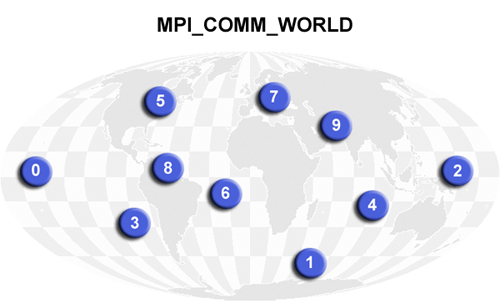
\includegraphics[width=0.5\textwidth]{./comm_world}      
      \end{center}
      \lstC{MPI_Comm_size(MPI_COMM_WORLD,int \&numtasks);}\\
      \lstC{MPI_Comm_rank(MPI_COMM_WORLD,int \&rank);}\\
      \vspace{0.5cm}
      \lstfortran{call MPI_COMM_SIZE(MPI_COMM_WORLD, numtasks, ierr)}\\
      \lstfortran{call MPI_COMM_RANK(MPI_COMM_WORLD, rank, ierr)}
    }
    \only<2->{
      \begin{itemize}
      \item Can be regarded as the name given to an ordered list of processes
      \item Each process has a unique rank, which starts from 0 
        (usually referred to as "root")
      \item It is the context of MPI communications and operations
        \begin{itemize}
        \item For instance, when a function is called to send data to all 
          processes, MPI needs to understand what "all" 
        \end{itemize}
      \item \lstC{MPI_COMM_WORLD}: the default communicator contains all processes 
        running a MPI program
      \item There can be many communicators
        \begin{itemize}
        \item e.g., \lstC{MPI_Comm_split(MPI_Commcomm, intcolor, int, kye, 
          MPI_Comm* newcomm)}
        \end{itemize}
      \item A process can belong to multiple communicators
        \begin{itemize}
        \item The rank is usually different
        \end{itemize}
      \end{itemize}
    }
  \end{itemize}
\end{frame}

\begin{frame}[fragile]
  \frametitle{Communicator Information}
  \begin{itemize}
  \item Rank: unique id of each process
    \begin{itemize}
    \item \textcolor{lubrown}{C:} \lstC{MPI_Comm_Rank(MPI_Comm comm, int *rank)}
    \item \textcolor{lubrown}{Fortran:} \lstfortran{MPI_COMM_RANK(COMM, RANK, ERR)}
    \end{itemize}
  \item Get the size/processes of a communicator
    \begin{itemize}
    \item \textcolor{lubrown}{C:} \lstC{MPI_Comm_Size(MPI_Comm comm, int *size)}
    \item \textcolor{lubrown}{Fortran:} \lstfortran{MPI_COMM_SIZE(COMM, SIZE, ERR)}
    \end{itemize}
  \end{itemize}
\end{frame}

\begin{frame}
  \frametitle{Compiling MPI Programs}
  \begin{itemize}
    \item Not a part of the standard
      \begin{itemize}
        \item Could vary from platform to platform
        \item Or even from implementation to implementation on the same  platform
        \item mpicc/mpicxx/mpif77/mpif90: wrappers to compile MPI code and auto 
          link to startup and message passing libraries 
      \end{itemize}
    \item<2> \alert<2>{Unlike OpenMP and OpenACC, you cannot compile a MPI program 
      for running in serial using the serial compiler}
    \item<2> \alert<2>{The MPI program is not a standard C/C++/Fortran program and 
      will split out errors about missing libraries} 
  \end{itemize}
\end{frame}

\begin{frame}[fragile, allowframebreaks]
  \frametitle{MPI Functions}
  \begin{itemize}
  \item Environment management functions
    \begin{enumerate}
    \item MPI\_INIT
    \item MPI\_COMM\_SIZE
    \item MPI\_COMM\_RANK
    \item MPI\_ABORT: Terminates all MPI processes
    \item MPI\_GET\_PROCESSOR\_NAME: Returns the processor name.
    \item MPI\_GET\_VERSION: Returns the version and subversion of the MPI standard
    \item MPI\_INITIALIZED: Indicates whether MPI\_Init has been called
    \item MPI\_WTIME: Returns an elapsed wall clock time in seconds
    \item MPI\_WTICK: Returns the resolution in seconds of MPI\_WTIME
    \item MPI\_FINALIZE
    \end{enumerate}
    \begin{columns}
      \column{0.4\textwidth}
      \begin{lstlisting}[language=C]
MPI_Init (&argc,&argv) 
MPI_Comm_size (comm,&size) 
MPI_Comm_rank (comm,&rank) 
MPI_Abort (comm,errorcode)
MPI_Get_processor_name (&name,&resultlength)
MPI_Get_version (&version,&subversion)
MPI_Initialized (&flag) 
MPI_Wtime ()
MPI_Wtick ()
MPI_Finalize ()
      \end{lstlisting}
      \column{0.4\textwidth}
      \begin{lstlisting}[language={[90]Fortran}]
MPI_INIT (ierr)
MPI_COMM_SIZE (comm,size,ierr)
MPI_COMM_RANK (comm,rank,ierr)
MPI_ABORT (comm,errorcode,ierr)
MPI_GET_PROCESSOR_NAME (name,resultlength,ierr)
MPI_GET_VERSION (version,subversion,ierr)
MPI_INITIALIZED (flag,ierr)
MPI_WTIME ()
MPI_WTICK ()
MPI_FINALIZE (ierr)
      \end{lstlisting}
    \end{columns}
    \framebreak
  \item Point-to-point communication functions
    \begin{itemize}
    \item Message transfer from one process to another
    \end{itemize}
  \item Collective communication functions 
    \begin{itemize}
    \item Message transfer involving all processes in a communicator
    \end{itemize}
  \end{itemize}
  \begin{columns}
    \column{0.4\textwidth}
    \begin{center}
      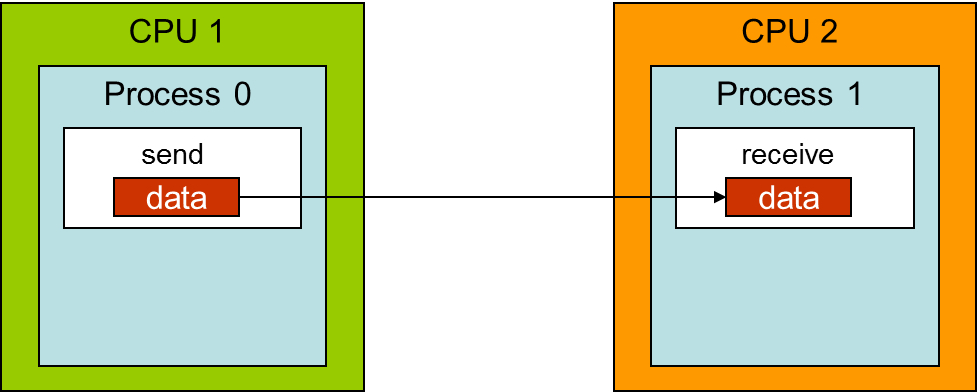
\includegraphics[width=\textwidth]{./SimpleSendAndRecv}
    \end{center}
    \column{0.4\textwidth}
    \begin{center}
      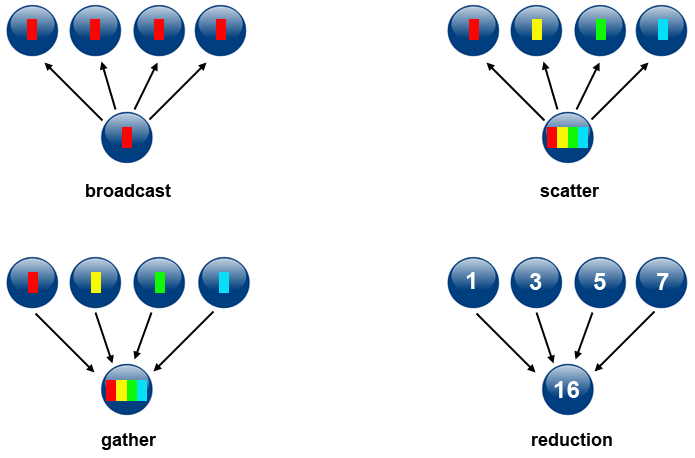
\includegraphics[width=\textwidth]{./collective_comm}
    \end{center}
  \end{columns}
\end{frame}

\begin{frame}[fragile, allowframebreaks]
  \frametitle{Point-to-point Communication}
  \begin{itemize}
  \item MPI point-to-point operations typically involve message passing between two, and only two, different MPI tasks. 
  \item One task is performing a send operation and the other task is performing a matching receive operation.
  \item There are different types of send and receive routines used for different purposes.
    \begin{enumerate}
    \item Blocking send / blocking receive
    \item Non-blocking send / non-blocking receive
    \item Synchronous send
    \end{enumerate}
  \end{itemize}

  \framebreak

  \begin{block}{Blocking vs. Non-blocking:}
    \begin{itemize}
    \item Blocking send / receive 
      \begin{itemize}
      \item send will "return" after it is safe to modify the application buffer (your send data) for reuse
      \item send can be synchronous i.e. handshake with the receive task to confirm a safe send.
      \item send can be asynchronous if a system buffer is used to hold the data for eventual delivery to the receive.
      \item receive only "returns" after the data has arrived and is ready for use by the program.
      \end{itemize}
    \item Non-blocking send / receive
      \begin{itemize}
      \item behave similarly - they will return almost immediately. 
      \item do not wait for any communication events to complete, such as message copying from user memory to system buffer space or the actual arrival of message.
      \item operations simply "request" the MPI library to perform the operation when it is able. 
      \item[] The user can not predict when that will happen.
      \item communications are primarily used to overlap computation with communication and exploit possible performance gains.
      \end{itemize}
    \end{itemize}
  \end{block}

  \framebreak
  
  \begin{block}{Blocking send / receive}
    \begin{itemize}
    \item \textbf{MPI\_Send}: Basic blocking send operation
    \item Routine returns only after the application buffer in the sending task is free for reuse.
    \item[] \lstC{MPI_Send (\&buf,count,datatype,dest,tag,comm) }
    \item[] \lstfortran{MPI_SEND (buf,count,datatype,dest,tag,comm,ierr)}
    \end{itemize}

    \begin{itemize}
    \item \textbf{MPI\_Recv}: Receive a message 
    \item will block until the requested data is available in the application buffer in the receiving task.
    \item[] \lstC{MPI_Recv (\&buf,count,datatype,source,tag,comm,\&status) }
    \item[] \lstfortran{MPI_RECV (buf,count,datatype,source,tag,comm,status,ierr)}
    \end{itemize}
  \end{block}
  
  \begin{block}{Non-blocking send / receive}
    \begin{itemize}
      \item \textbf{MPI\_Isend}: Identifies an area in memory to serve as a send buffer.
      \item Processing continues immediately without waiting for the message to be copied out from the application buffer
      \item[] \lstC{MPI_Isend (\&buf,count,datatype,dest,tag,comm,\&request) }
      \item[] \lstfortran{MPI_ISEND (buf,count,datatype,dest,tag,comm,request,ierr)}
      \item \textbf{MPI\_Irecv}: Identifies an area in memory to serve as a receive buffer
      \item Processing continues immediately without actually waiting for the message to be received and copied into the the application buffer
      \item[] \lstC{MPI_Irecv (\&buf,count,datatype,source,tag,comm,\&request)}
      \item[] \lstfortran{MPI_IRECV (buf,count,datatype,source,tag,comm,request,ierr)}
      \item \textbf{MPI\_WAIT} and \textbf{MPI\_TEST}: Functions required by nonblocking send and receive use to determine when the non-blocking receive operation completes and the requested message is available in the application buffer.
    \end{itemize}
  \end{block}

  \begin{block}{Synchronous send}
    \begin{itemize}
    \item \textbf{MPI\_Ssend}: Send a message 
    \item will block until the application buffer in the sending task is free for reuse and the destination process has started to receive the message.
    \item[] \lstC{MPI_Ssend (\&buf,count,datatype,dest,tag,comm) }
    \item[ ]\lstfortran{MPI_SSEND (buf,count,datatype,dest,tag,comm,ierr)}
%    \item \textbf{MPI\_Sendrecv}: Send a message and post a receive before blocking
%    \item Will block until the sending application buffer is free for reuse and until the receiving application buffer contains the received message.
%    \item[] \lstC{MPI_Sendrecv (\&sendbuf,sendcount,sendtype,dest,sendtag,\&recvbuf,recvcount,recvtype,source,recvtag,comm,\&status) }
%    \item[] \lstfortran{MPI_SENDRECV (sendbuf,sendcount,sendtype,dest,sendtag,recvbuf,recvcount,recvtype,source,recvtag,comm,status,ierr)}
    \item \textbf{MPI\_Issend}: Non-blocking synchronous send
    \item[] \lstC{MPI_Issend (\&buf,count,datatype,dest,tag,comm,\&request) }
    \item[] \lstfortran{MPI_ISSEND (buf,count,datatype,dest,tag,comm,request,ierr)}
    \end{itemize}
  \end{block}
\end{frame}

\begin{frame}[fragile,allowframebreaks]
  \frametitle{Blocking Message Passing Example}
    \begin{columns}
      \column{0.45\textwidth}
      \lstinputlisting[basicstyle=\fontsize{3.5}{4.5}\selectfont\ttfamily,language=C]{./src/mpi/pingpong.c}
      \column{0.45\textwidth}
      \lstinputlisting[basicstyle=\fontsize{3.5}{4.5}\selectfont\ttfamily,language={[90]Fortran}]{./src/mpi/pingpong.f90}
    \end{columns}
    \framebreak
    \begin{columns}
      \column{0.45\textwidth}
      \lstinputlisting[basicstyle=\fontsize{3.5}{4.5}\selectfont\ttfamily,language=C]{./src/mpi/ring.c}
      \column{0.45\textwidth}
      \lstinputlisting[basicstyle=\fontsize{3.5}{4}\selectfont\ttfamily,language={[90]Fortran}]{./src/mpi/ring.f90}
    \end{columns}
  \framebreak
  \begin{exampleblock}{}
    \begin{lstlisting}
[alp514.sol](1110): mpicc -o ringc ring.c
[alp514.sol](1113): srun -p eng -n 4 ./ringc
Task 0: Received from task 3 with tag 1 and from task 1 with tag 2
Task 0: Send to task 3 with tag 2 and to task 1 with tag 1
Task 1: Received from task 0 with tag 1 and from task 2 with tag 2
Task 1: Send to task 0 with tag 2 and to task 2 with tag 1
Task 2: Received from task 1 with tag 1 and from task 3 with tag 2
Task 2: Send to task 1 with tag 2 and to task 3 with tag 1
Task 3: Received from task 2 with tag 1 and from task 0 with tag 2
Task 3: Send to task 2 with tag 2 and to task 0 with tag 1
    \end{lstlisting}
  \end{exampleblock}{}
  \begin{exampleblock}{}
    \begin{lstlisting}
[alp514.sol](1111): mpif90 -o ringf ring.f90
[alp514.sol](1114): srun -p eng -n 4 ./ringf
Task  3: Received from task 2 with tag 1 and from task 0 with tag 2
Task  3: Send to task 2 with tag 2 and to task 0 with tag 1
Task  0: Received from task 3 with tag 1 and from task 1 with tag 2
Task  0: Send to task 3 with tag 2 and to task 1 with tag 1
Task  1: Received from task 0 with tag 1 and from task 2 with tag 2
Task  1: Send to task 0 with tag 2 and to task 2 with tag 1
Task  2: Received from task 1 with tag 1 and from task 3 with tag 2
Task  2: Send to task 1 with tag 2 and to task 3 with tag 1
    \end{lstlisting}
  \end{exampleblock}
\end{frame}

\begin{frame}{Further Reading}
  \begin{itemize}
    \item Tutorials
    \begin{enumerate}
      \item MPI: \url{https://computing.llnl.gov/tutorials/mpi/}
      \item Advanced MPI: \url{https://hpc.llnl.gov/sites/default/files/DavidCronkSlides.pdf}
      \item CITutor: \url{https://www.citutor.org/}
      \item XSEDE HPC Monthly Workshop Series: \url{https://psc.edu/xsede-hpc-series-all-workshops}
      \item MPI Tutorial: \url{http://mpitutorial.com/}
    \end{enumerate}
    \item Books
    \begin{enumerate}
      \item Beginning MPI (An Introduction in C) by Wesley Kendall
      \item Parallel Programming with MPI by Peter Pacheco (No relation)
      \item Using MPI - 2nd Edition: Portable Parallel Programming with the Message Passing Interface (Scientific and Engineering Computation) by William Gropp
      \item Parallel Programming in C with MPI and Openmp by Michael J. Quinn
      \item MPI: The Complete Reference by Marc Snir \textit{et. al.}
    \end{enumerate}
  \end{itemize}
\end{frame}

\end{document}

